% Created by tikzDevice version 0.12.3.1 on 2021-11-16 08:52:24
% !TEX encoding = UTF-8 Unicode
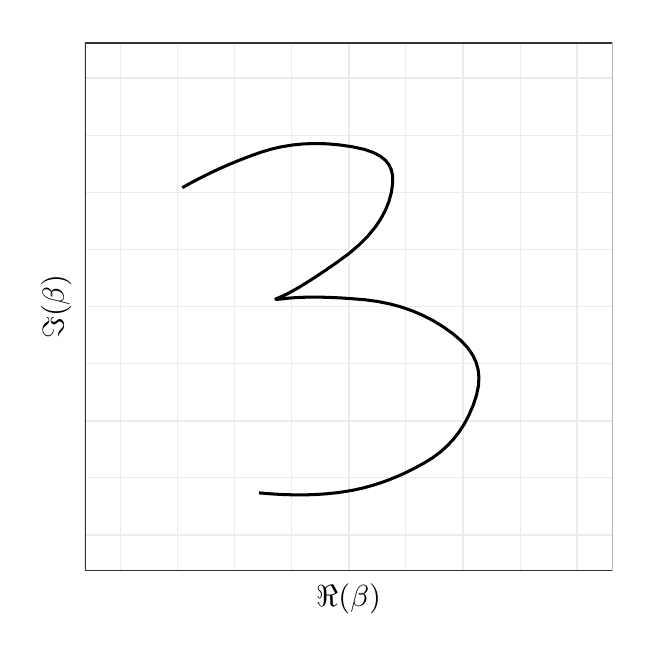
\begin{tikzpicture}[x=1pt,y=1pt]
\definecolor{fillColor}{RGB}{255,255,255}
\path[use as bounding box,fill=fillColor,fill opacity=0.00] (0,0) rectangle (216.81,216.81);
\begin{scope}
\path[clip] (  0.00,  0.00) rectangle (216.81,216.81);
\definecolor{drawColor}{RGB}{255,255,255}
\definecolor{fillColor}{RGB}{255,255,255}

\path[draw=drawColor,line width= 0.6pt,line join=round,line cap=round,fill=fillColor] (  0.00,  0.00) rectangle (216.81,216.81);
\end{scope}
\begin{scope}
\path[clip] ( 20.71, 20.71) rectangle (211.31,211.31);
\definecolor{fillColor}{RGB}{255,255,255}

\path[fill=fillColor] ( 20.71, 20.71) rectangle (211.31,211.31);
\definecolor{drawColor}{gray}{0.92}

\path[draw=drawColor,line width= 0.3pt,line join=round] ( 20.71, 54.13) --
	(211.31, 54.13);

\path[draw=drawColor,line width= 0.3pt,line join=round] ( 20.71, 95.38) --
	(211.31, 95.38);

\path[draw=drawColor,line width= 0.3pt,line join=round] ( 20.71,136.64) --
	(211.31,136.64);

\path[draw=drawColor,line width= 0.3pt,line join=round] ( 20.71,177.89) --
	(211.31,177.89);

\path[draw=drawColor,line width= 0.3pt,line join=round] ( 54.13, 20.71) --
	( 54.13,211.31);

\path[draw=drawColor,line width= 0.3pt,line join=round] ( 95.38, 20.71) --
	( 95.38,211.31);

\path[draw=drawColor,line width= 0.3pt,line join=round] (136.64, 20.71) --
	(136.64,211.31);

\path[draw=drawColor,line width= 0.3pt,line join=round] (177.89, 20.71) --
	(177.89,211.31);

\path[draw=drawColor,line width= 0.6pt,line join=round] ( 20.71, 33.50) --
	(211.31, 33.50);

\path[draw=drawColor,line width= 0.6pt,line join=round] ( 20.71, 74.76) --
	(211.31, 74.76);

\path[draw=drawColor,line width= 0.6pt,line join=round] ( 20.71,116.01) --
	(211.31,116.01);

\path[draw=drawColor,line width= 0.6pt,line join=round] ( 20.71,157.27) --
	(211.31,157.27);

\path[draw=drawColor,line width= 0.6pt,line join=round] ( 20.71,198.52) --
	(211.31,198.52);

\path[draw=drawColor,line width= 0.6pt,line join=round] ( 33.50, 20.71) --
	( 33.50,211.31);

\path[draw=drawColor,line width= 0.6pt,line join=round] ( 74.76, 20.71) --
	( 74.76,211.31);

\path[draw=drawColor,line width= 0.6pt,line join=round] (116.01, 20.71) --
	(116.01,211.31);

\path[draw=drawColor,line width= 0.6pt,line join=round] (157.27, 20.71) --
	(157.27,211.31);

\path[draw=drawColor,line width= 0.6pt,line join=round] (198.52, 20.71) --
	(198.52,211.31);
\definecolor{drawColor}{RGB}{0,0,0}

\path[draw=drawColor,line width= 1.1pt,line join=round] ( 83.58, 48.71) --
	( 88.21, 48.33) --
	( 92.63, 48.09) --
	( 96.83, 47.98) --
	(100.83, 48.00) --
	(104.64, 48.14) --
	(108.27, 48.40) --
	(111.72, 48.76) --
	(115.00, 49.23) --
	(118.13, 49.79) --
	(121.20, 50.48) --
	(124.28, 51.31) --
	(127.36, 52.28) --
	(130.45, 53.39) --
	(133.56, 54.65) --
	(136.70, 56.06) --
	(139.86, 57.63) --
	(143.04, 59.37) --
	(146.15, 61.27) --
	(148.96, 63.35) --
	(151.50, 65.61) --
	(153.81, 68.06) --
	(155.89, 70.72) --
	(157.77, 73.62) --
	(159.45, 76.79) --
	(160.93, 80.25) --
	(162.21, 84.05) --
	(162.89, 87.44) --
	(163.05, 90.51) --
	(162.75, 93.33) --
	(161.99, 95.99) --
	(160.77, 98.57) --
	(159.00,101.13) --
	(156.61,103.71) --
	(153.48,106.35) --
	(150.02,108.81) --
	(146.45,110.98) --
	(142.76,112.87) --
	(138.94,114.51) --
	(134.96,115.89) --
	(130.79,117.01) --
	(126.42,117.88) --
	(121.83,118.49) --
	(117.20,118.88) --
	(112.94,119.16) --
	(109.03,119.34) --
	(105.47,119.44) --
	(102.23,119.45) --
	( 99.29,119.38) --
	( 96.64,119.25) --
	( 94.26,119.06) --
	( 92.14,118.81) --
	( 90.79,118.70) --
	( 90.04,118.66) --
	( 89.72,118.68) --
	( 89.64,118.71) --
	( 89.64,118.74) --
	( 89.77,118.82) --
	( 90.18,119.02) --
	( 91.06,119.37) --
	( 92.32,119.91) --
	( 93.89,120.67) --
	( 95.80,121.70) --
	( 98.11,123.02) --
	(100.83,124.69) --
	(104.01,126.73) --
	(107.69,129.18) --
	(111.89,132.09) --
	(116.24,135.30) --
	(119.92,138.47) --
	(123.00,141.59) --
	(125.55,144.67) --
	(127.62,147.75) --
	(129.26,150.83) --
	(130.51,153.96) --
	(131.39,157.16) --
	(131.90,160.48) --
	(131.88,163.17) --
	(131.43,165.38) --
	(130.57,167.24) --
	(129.28,168.87) --
	(127.47,170.34) --
	(124.99,171.66) --
	(121.66,172.83) --
	(117.28,173.78) --
	(112.64,174.45) --
	(108.18,174.84) --
	(103.88,174.95) --
	( 99.71,174.81) --
	( 95.67,174.41) --
	( 91.73,173.77) --
	( 87.87,172.88) --
	( 84.08,171.74) --
	( 80.35,170.40) --
	( 76.69,168.99) --
	( 73.08,167.51) --
	( 69.53,165.95) --
	( 66.04,164.32) --
	( 62.60,162.62) --
	( 59.22,160.85) --
	( 55.88,159.00) --
	( 55.88,159.00);
\definecolor{drawColor}{gray}{0.20}

\path[draw=drawColor,line width= 0.6pt,line join=round,line cap=round] ( 20.71, 20.71) rectangle (211.31,211.31);
\end{scope}
\begin{scope}
\path[clip] (  0.00,  0.00) rectangle (216.81,216.81);
\definecolor{drawColor}{RGB}{0,0,0}

\node[text=drawColor,anchor=base,inner sep=0pt, outer sep=0pt, scale=  1.10] at (116.01,  7.64) {$\Re(\beta)$};
\end{scope}
\begin{scope}
\path[clip] (  0.00,  0.00) rectangle (216.81,216.81);
\definecolor{drawColor}{RGB}{0,0,0}

\node[text=drawColor,rotate= 90.00,anchor=base,inner sep=0pt, outer sep=0pt, scale=  1.10] at ( 13.08,116.01) {$\Im(\beta)$};
\end{scope}
\end{tikzpicture}
